\documentclass[./../../paper.tex]{subfiles}
\graphicspath{{\subfix{./../../figures/}}}

\begin{document}

In this comparison, we employ the baseline models mentioned in \autoref{sec:model_generation}. Namely, the \emph{Case-Based Generator}, the \emph{Sample-Based Generator} and the \emph{Random Generator}. 

We randomly sample \optional{20} factuals from the test set and use the same factuals for every generator. We ensure, that the outcomes are evenly divided. The remaining procedure follows the established procedure of previous experiments.

\begin{figure}[htbp]
    \centering
    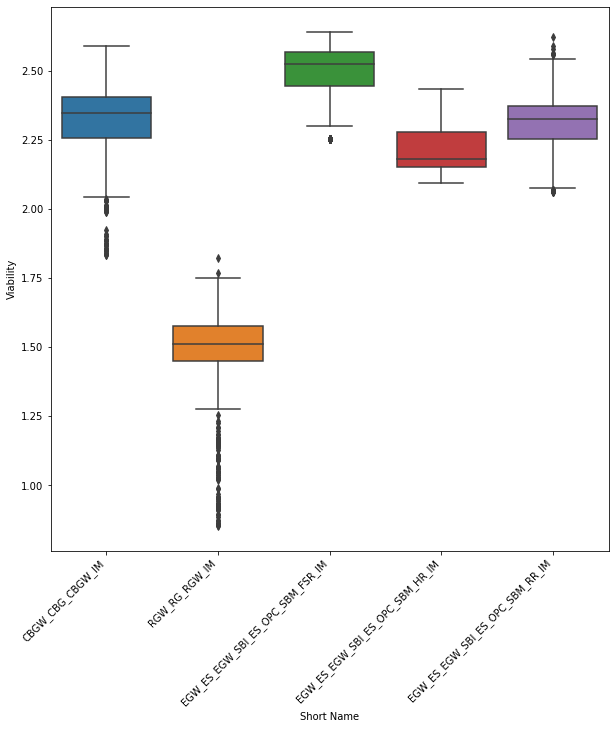
\includegraphics[width=\textwidth]{figures/generated/exp4_winner_overall.png}
    \caption{This figure shows boxplots of the viability of each models' generated counterfactual.}
    \label{fig:exp4-winner}
\end{figure}

\noindent The results shown in \autoref{fig:exp4-winner} show that the evolutionary algorithm \optional{CBI-ES-UC3-SBM-RR} slightly returns better results when it comes to the median viability. The worst model is the random generated model. The Case-Based model appears to be evenly and normally distributed at a viability of \optional{2.25}. The \optional{CBI-RWS-OPC-SBM-FSR} has outliers that far exceed or underperform against other evolutionary algorithms. 

\autoref{fig:exp4-winner} also displays the vast difference in computation time for the evoulutionary algorithms. Only the model using the \optional{Ranking-Recombination} reranking version seems to be slightly faster than the ones using Best-Breed and Fittest-Survivor as recombination methods.

\autoref{tbl:exp4-winner} shows the detailed results.

\begin{table}
    \caption{Table shows the result of Experiment 4. The colors indicate the model configurations that were examined. The results are based on the average viability each counterfactual a model produces across all factuals that were tested.}
    \label{tbl:exp4-winner}
\makebox[\linewidth]{

\begin{table}
\caption{Table shows the result of Experiment 4. The colors indicate the model configurations that were examined. The results are based on the average viability each counterfactual a model produces across all factuals that were tested.}
\label{tbl:exp4-winner}
\begin{tabular}{lrrrrrrrrrrrrrrrr}
 & experiment & Rank & Prediction Score & Viability & Sparcity & Similarity & Feasibility & Delta & cf-num-zeros & result-outcome & source-outcome & target-outcome & Processing Time (sec.) & run.mask & run.no & wrapper.max-len \\
Model (Abbr. Name) &  &  &  &  &  &  &  &  &  &  &  &  &  &  &  &  \\
CBG-CBGW & 1.000000 & 25.500000 & 0.514867 & 2.230507 & 0.764022 & 0.818115 & 0.014585 & 0.633786 & 14.584000 & 0.324000 & 0.500000 & 0.500000 & 9.414627 & 1111.000000 & 1.000000 & 27.000000 \\
CBI-ES-UC3-SBM-RR & 1.000000 & 25.500000 & 0.497746 & 2.678977 & 0.870874 & 0.896964 & 0.087737 & 0.823403 & 15.448000 & 0.500000 & 0.500000 & 0.500000 & 588.550365 & 1111.000000 & 4.000000 & 27.000000 \\
CBI-RWS-OPC-SBM-BBR & 1.000000 & 25.500000 & 0.445966 & 2.612767 & 0.851280 & 0.882271 & 0.095409 & 0.783807 & 15.560000 & 0.384000 & 0.500000 & 0.500000 & 631.307437 & 1111.000000 & 6.000000 & 27.000000 \\
CBI-RWS-OPC-SBM-FSR & 1.000000 & 25.500000 & 0.463966 & 2.728961 & 0.870071 & 0.899039 & 0.160373 & 0.799478 & 15.432000 & 0.500000 & 0.500000 & 0.500000 & 625.714404 & 1111.000000 & 5.000000 & 27.000000 \\
RG-RGW & 1.000000 & 25.500000 & 0.569685 & 1.554904 & 0.338077 & 0.578003 & 0.000000 & 0.638824 & 1.034000 & 0.432000 & 0.500000 & 0.500000 & 8.175288 & 1111.000000 & 2.000000 & 27.000000 \\
SBG-SBGW & 1.000000 & 25.500000 & 0.487669 & 2.151321 & 0.717582 & 0.755577 & 0.171964 & 0.506198 & 25.016000 & 0.016000 & 0.500000 & 0.500000 & 9.927904 & 1111.000000 & 3.000000 & 27.000000 \\
\end{tabular}
\end{table}

}
\end{table}


\end{document}